\section{Results}
\label{sec:results}

\begin{figure}
\centering
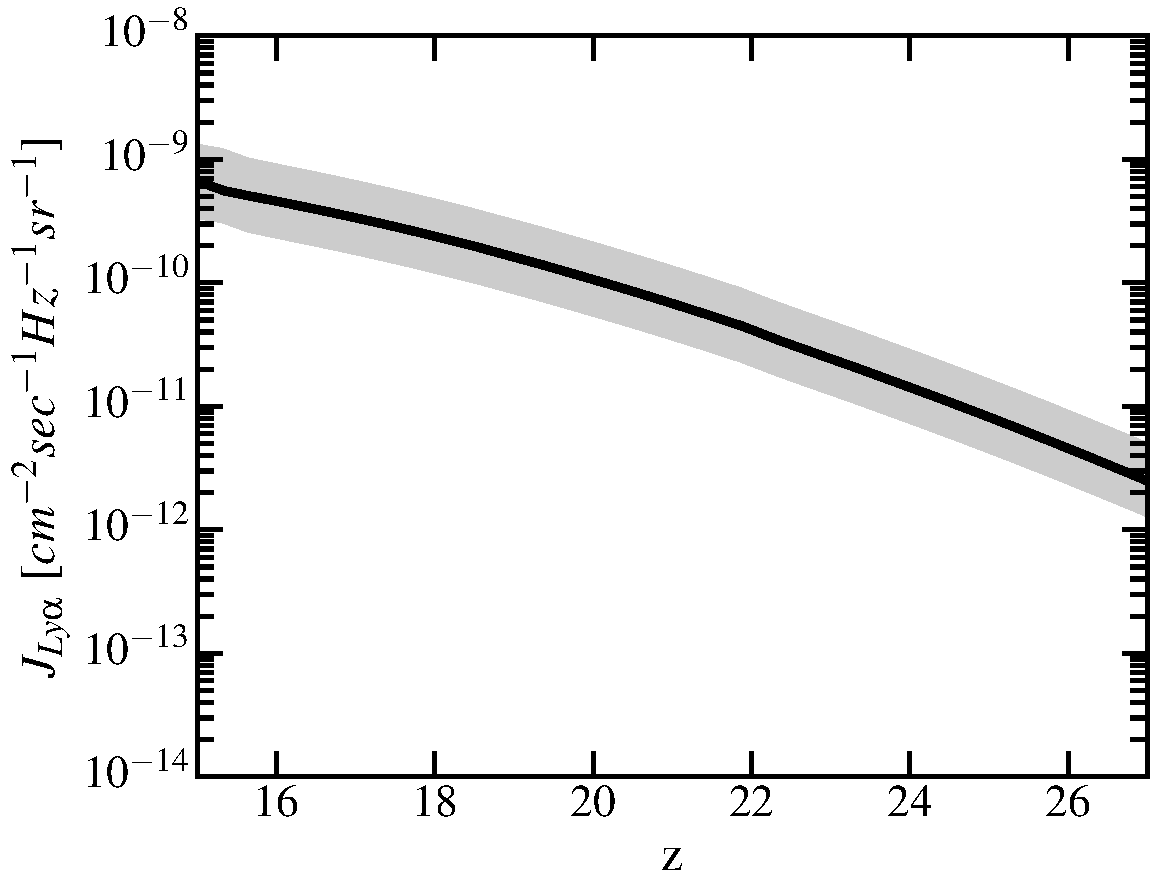
\includegraphics[width=.35\textwidth,keepaspectratio=true]{Jlya.pdf}
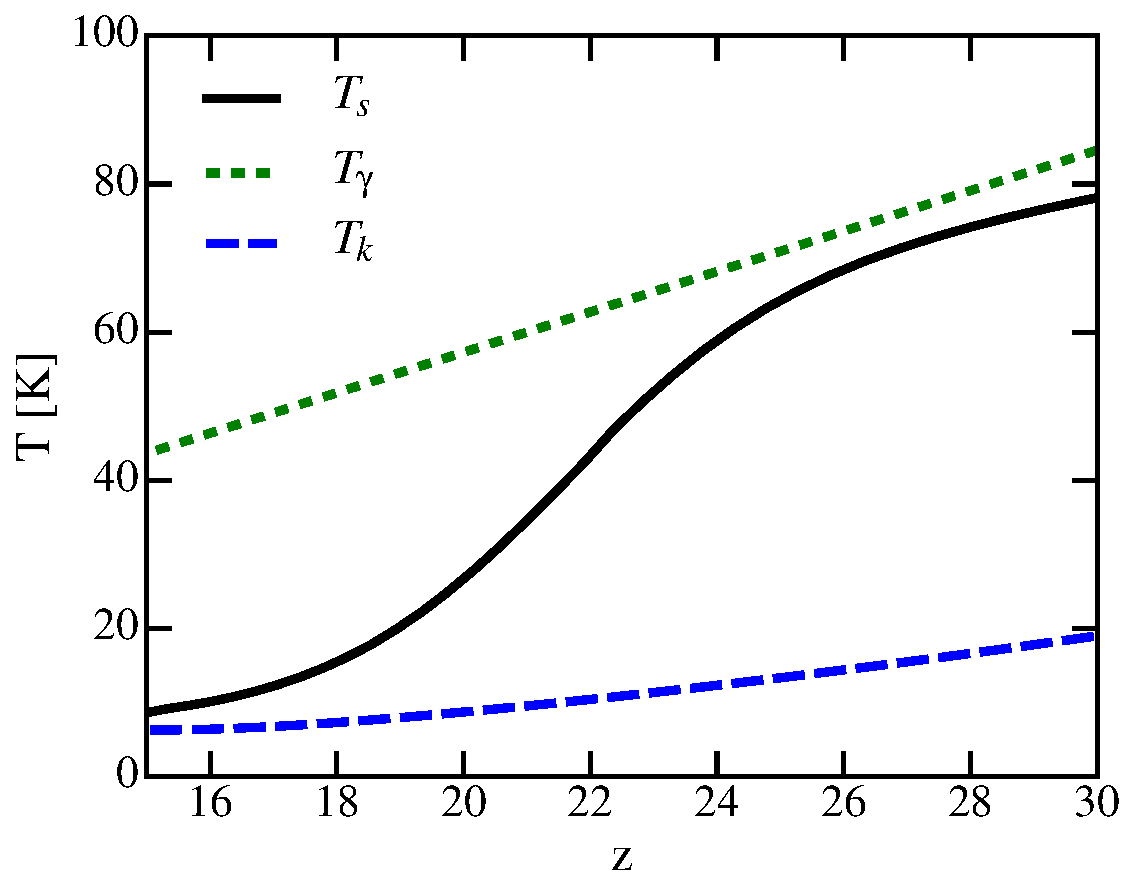
\includegraphics[width=.35\textwidth,keepaspectratio=true]{Ts.pdf}
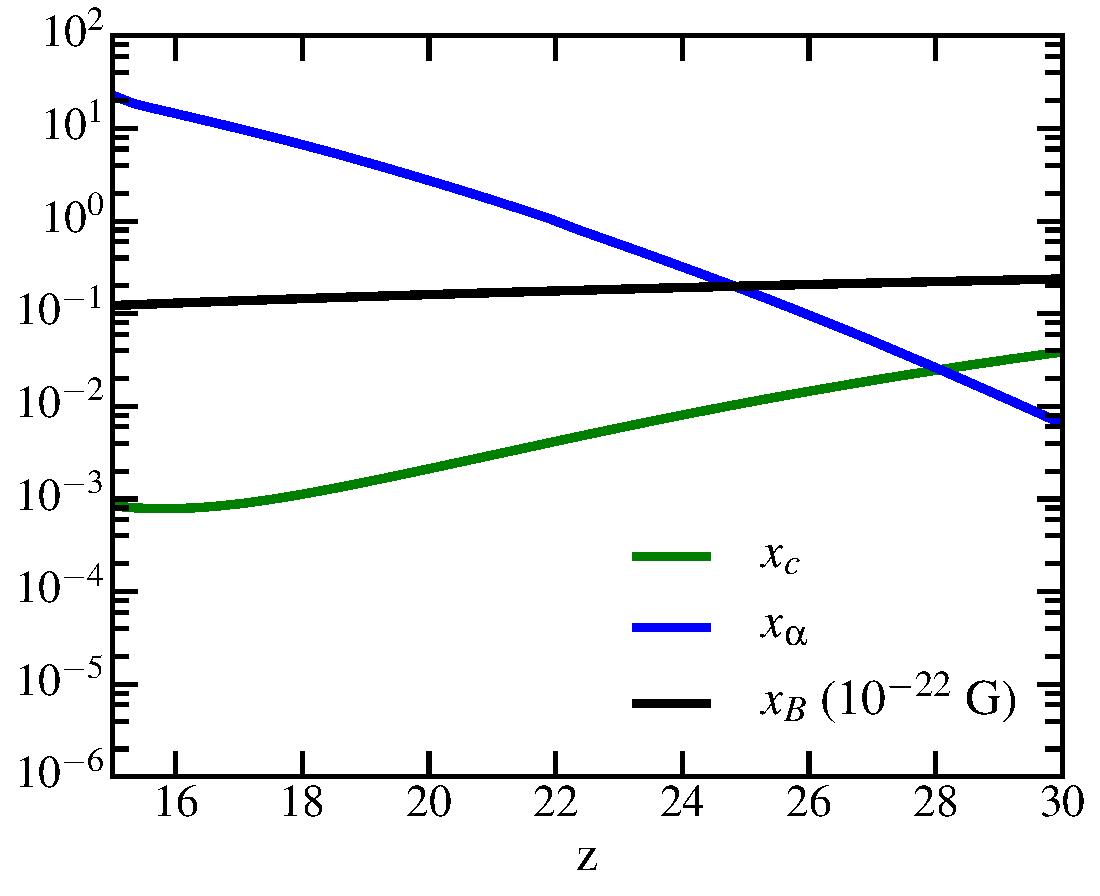
\includegraphics[width=.35\textwidth,keepaspectratio=true]{xs.pdf}
\caption{Inputs used for the sensitivity calculation, computed for standard cosmology using \texttt{21CMFAST} code. Top panel: Lyman-$\alpha$ flux model; fiducial choice used for sensitivity calculations is shown with a solid line, while the extrema of the gray band are used to test the effects of the uncertainty in the Lyman--$\alpha$ flux at high redshift (as discussed in the text). Middle panel: fiducial models for spin, kinetic, and CMB temperatures. Bottom panel: fiducial models for quantities that parametrize the rate of depolarization of the ground state by optical pumping and atomic collisions, and the rate of magnetic precession for a representative value of the magnetic field. \label{fig:cosmo}}
\end{figure}
We now proceed to numerically evaluate the sensitivity of 21--cm tomography to magnetic fields during the pre--reionization epoch, using the formalism from previous two Sections. For this purpose, we only focus on one type of experimental setup---an array of dipole antennas arranged in a compact grid. The motivation for this choice is that such a configuration maximizes sensitivity to recovering the power spectrum of the cosmological 21--cm signal \cite{2009PhRvD..79h3530T,2015AAS...22532803D}. We consider an array with a collecting area of $(\Delta L\text{ km})^2$, where $\Delta L$ is taken to be the maximal baseline separation. In this case, the observation time $t_1$ entering the expression for the noise of Eq.~(\ref{eq:Pnoise_K}) is the same as the total survey duration\footnote{Calculation of the observation time $t_1$, given total survey duration $t_\text{obs}$, depends on the type of the experiment. For a radio dish with a beam of solid angle $\Omega_\text{beam}=\lambda^2/A_e$ (smaller than the survey size $\Omega_\text{survey}$), where the telescope scans the sky one beamwidth at a time, $t_1$ is the total time spent observing one $(u,v)$ element, and thus $t_1=t_\text{obs}\Omega_\text{survey}/\Omega_\text{beam}$.}, $t_1=t_\text{obs}$. We do not explicitly account for the fact that any given portion of the sky is above the horizon of a given location only for a part of a day; therefore, $t_\text{obs}$ we substitute in the noise calculation is shorter than the corresponding wall--clock duration of the survey (by a factor equal to the fraction of the day that a given survey region is above the horizon). To derive numerical results, we assume $\Omega_\text{survey}=1$sr and $t_\text{obs}=1$ year (corresponding to the wall--clock observing time on the order of three years). To compute sky temperature, we assume a simple model for Galactic synchrotron emission from Ref.~\cite{2008PhRvD..78b3529M}, 
\beq
T_\text{sky}  = 60\left(\frac{21}{100} (1+z)\right)^{2.55}\text{   [K]}.
\label{eq:tsys}
\eeq
We take the observed redshift range to be $z\in[15,30]$. 

Other inputs to the sensitivity calculation are all shown in Fig.~\ref{fig:cosmo}: the mean Lyman--$\alpha$ flux $J_{\text{Ly}\alpha}$ as a function of redshift (top panel); the spin $T_s$ and kinetic $T_k$ temperatures of the IGM, along with the CMB $T_\gamma$ temperature, also as functions of redshift (middle panel); and the quantities that parametrize the rate of depolarization of the ground state by optical pumping $x_{\alpha,(2)}$ and atomic collisions $x_{c,(2)}$, and the rate of magnetic precession $x_B$ for a representative value of the magnetic field. We obtain the quantities from top two panels from \texttt{21CMFAST} code \cite{2011MNRAS.411..955M}. As input to \texttt{21CMFAST}, we use standard cosmological parameters ($H_0=67$ km s$^{-1}$ Mpc$^{-1}$, $\Omega_\text{m}=0.32$, $\Omega_K=0$, $n_s=0.96$, $\sigma_8=0.83$, $w=-1$) consistent with Planck measurements \cite{2015arXiv150201589P}. We set the sources responsible for early heating to Population III stars by setting \verb|Pop|$=3$, and keep all other input parameters at their default values, with the exception of the star formation efficiency, \verb|F_STAR|. For our fiducial calculation (denoted with solid curves in Fig.~\ref{fig:cosmo}), we choose \verb|F_STAR|=$0.014897$, but we also explore two other reionization models, as discussed below. The fiducial model is chosen to match the models from Ref.~\cite{2012ApJ...746..125H} at $z=15$ (which were computed by extrapolation of the flux measurements from observations at much lower redshifts). We tested that this fiducial model is physically reasonable, in the sense that it produces a sufficient number of ionizing photons to reionize the universe; we detail these tests in Appendix \ref{app:fesc}. 

Since the evolution of the Lyman--$\alpha$ flux prior to reionization is unconstrained by observations, we vary our input flux model (and, correspondingly, the models for the temperaures and depolarization rates, etc.) in order to capture the effect of this uncertainty on the key results of our sensitivity calculation. Specifically, we consider two ``extreme'' models for the Lyman--$\alpha$ flux, shown in the top panel of Fig.~\ref{fig:cosmo} as the extrema of the gray band of ``uncertainty'' around the fiducial $J_{\text{Ly}\alpha}(z)$ curve. They are obtained from \texttt{21CMFAST} runs with twice (for the top edge of the gray band), and one half (bottom edge) the fiducial value of \verb|F_STAR|.  Note that the rest of the panels in this Figure only show the fiducial model in order to avoid clutter, but the corresponding variation in all quantities is consistently included in our calculation. 

\begin{figure}
\centering
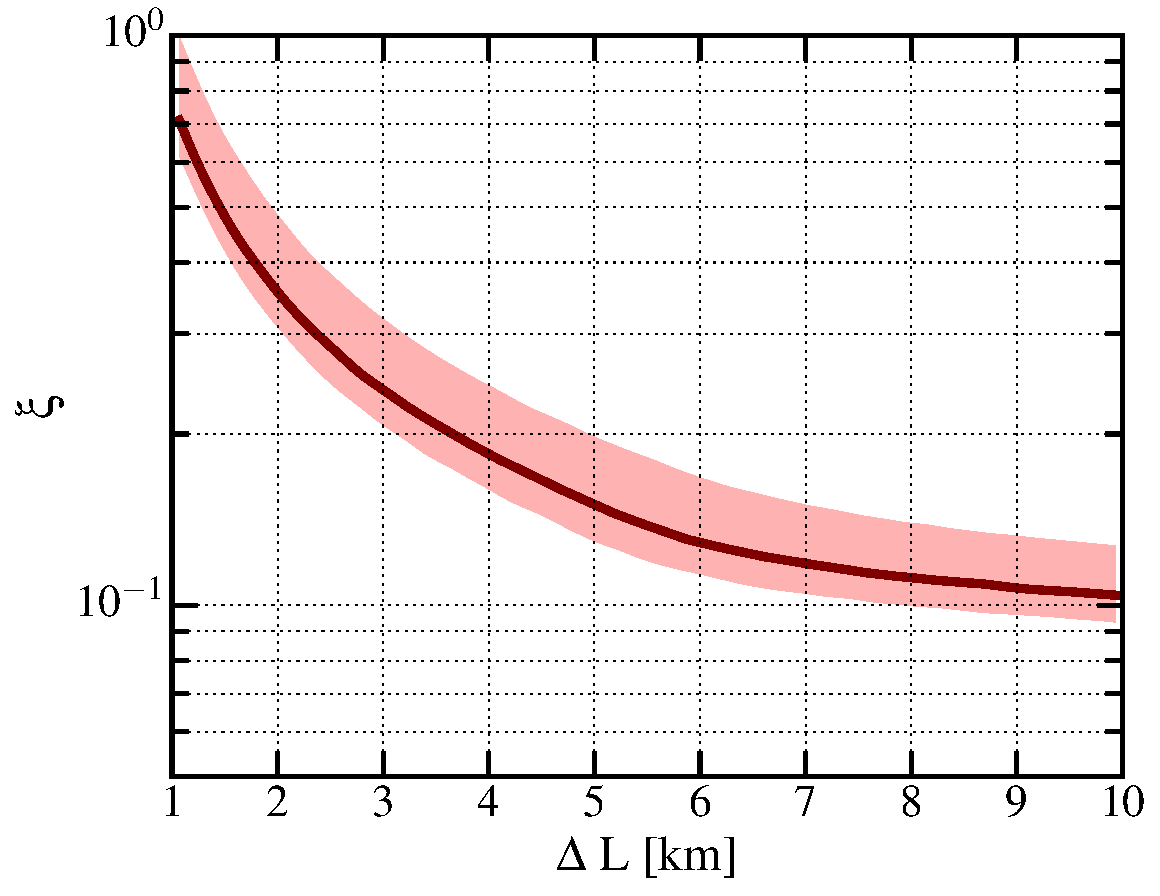
\includegraphics[width=.35\textwidth,keepaspectratio=true]{xi_vs_deltas.pdf}
\caption{Projected sensitivity to detecting a magnetic field in the saturated regime, as a function of the maximum baseline (or, equivalently, of the total collecting area, ($\Delta L)^2$), assuming a survey size of 1 sr and a total observation time of three years. The parameter on the $y$ axis characterizes the distinction between the case of no magnetic field ($\xi=0$) and a strong magnetic field ($\xi=1$). Smaller values here (for larger maximum--baseline values shown on the $x$ axis) correspond to more sensitivity to recovering $\xi$, and thus to better prospect for distinction between the two regimes. The light--colored band around the solid line corresponds to the Lyman--$\alpha$ model flux uncertainty, represented with a gray band in Fig.~\ref{fig:cosmo}.\label{fig:xi_vs_deltas}}
\end{figure}
\begin{figure}
\centering
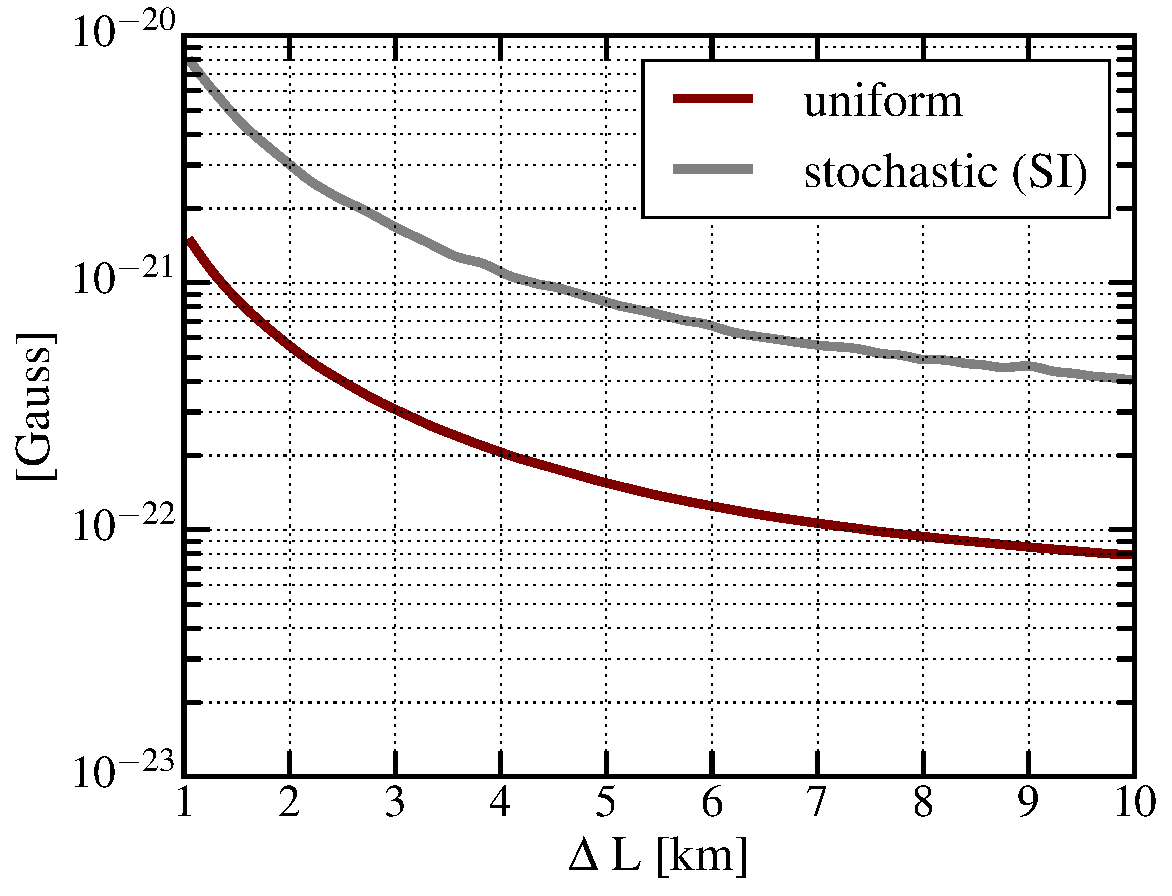
\includegraphics[width=.35\textwidth,keepaspectratio=true]{B_vs_deltas.pdf}
\caption{Projected $1\sigma$ sensitivity to detecting a uniform (lower red line) and a stochastic (upper gray line) magnetic field, as a function of maximum baseline $\Delta L$ (the collecting area of the array is given as $(\Delta L)^2$).  For the stochastic field, we assume a scale--invariant (SI) power spectrum, and show here the sensitivity to the root--mean--square variation per $\log K$, or $A_0/\pi$, where $A_0^2$ is the amplitude of the power in a transverse component of the field. We assume a survey size of 1 sr and a total observing time of three years.\label{fig:B_vs_deltas}}
\end{figure}
Figs.~\ref{fig:xi_vs_deltas} and \ref{fig:B_vs_deltas} show the key results: the projected sensitivity of tomographic surveys as a function of the maximum baseline $\Delta L$ (where different values of $\Delta L$ may correspond to different stages of a single experiment). Fig.~\ref{fig:xi_vs_deltas} shows $1\sigma$ sensitivity to parameter $\xi$ of \eq{\ref{eq:saturated_P}} which quantifies the level of distinction between the case of no magnetic field and the case where the field is strong and the signal is in the saturated regime. The value of this parameter is, by definition, bound between 0 and 1, representing, respectively, the case of no magnetic field and the saturated case. In this Figure, the solid line represents our fiducial calculation, while the light--colored band around it corresponds to the level of variation in the input Lyman--$\alpha$ flux shown as a grey band in Fig.~\ref{fig:cosmo}. The fiducial result implies that an array of dipoles with one--kilometer--squared collecting area can achieve $1\sigma$ sensitivity to detecting a magnetic field in signal--saturation regime. Such detection of non--vanishing value of $\xi$ can then be interpreted as a lower bound on a uniform magnetic field, at a a $1\sigma$ confidence level (assuming the field is uniform in the entire survey volume). The value of the lower bound as a function of redshift  corresponds, in this case, to the saturation ``ceiling'' at that redshift, which can be roughly evaluated by requiring that the depolarization rates through standard channels equal the rate of magnetic precession, $x_B = 1+x_{\alpha ,(2)} +x_{c,(2)}$. The ceiling is depicted with a dashed line in Fig.~\ref{fig:Bsat}, and it corresponds to $|\vec B|\sim 2\times 10^{-21}$ Gauss (comoving) at $z=20$, for example.  On the other hand, if a survey were to report a null result, it would rule out such a magnetic field, at the same confidence level. In this case, the result would imply an upper bound on the strength of the magnetic field components in the plane of the sky, as discussed in the following. 

We obtain results in Fig.~\ref{fig:B_vs_deltas} by evaluating the expressions of Eqs.~(\ref{eq:fisher_patch}) and (\ref{eq:snr_ints}). This Figure shows a projected $1\sigma$ upper bound that can be placed on the value of the magnetic field, in case of no detection with an array of a given size. The result is shown for both the uniform field (lower solid red line), and for the amplitude of a stochastic field (upper gray line) with a scale--independent power spectrum. It implies that an array with one square kilometer collecting area may be able to detect a field of strength $10^{-21}$ Gauss comoving, at $1\sigma$ confidence level, after three years of observation.

While the numerical calculation assumed that the brightness temperature is a linear function of the field strength, this assumption is not guaranteed to hold---it breaks down in the limit of a strong field, as discussed above and in \S\ref{sec:method}. So, the results of this Figure are only valid if the value of the $\xi$ parameter is small. In order to demonstrate how these projected constraints (sensitivities) compare to the saturation ceiling, Fig.~\ref{fig:Bsat} shows a comparison between the saturation ceiling and the values of the integrand of \eq{\ref{eq:fisher_patch}} (plotted for several array sizes, as a function of redshift). From that Figure, we see that the sensitivity to the uniform field corresponding to arrays with collecting areas slightly above a kilometer squared lies below the saturation ceiling for redshifts contributing most of the signal--to--noise, $z\sim21$ (the minima of these curves). This gives us confidence that the results for the uniform field in Fig.~\ref{fig:B_vs_deltas} are indeed valid, and the linear theory holds in the given regime (the transfer function is a linear function of the field strength). For the stochastic case, however, it is likely that a factor of a few larger array sizes are needed to achieve sensitivity that is below the saturation ceiling at relevant redshifts. It is important to note two things here. First, the saturation ceiling presented in this Figure is quite conservatively calculated, while, in reality, the linear approximation may hold for field strengths a few times above this level. Second, a downwards variation of the Lyman--$\alpha$ flux by a factor of a few from our fiducial value at redshift of $\sim 21$ can easily change relative values of the ceiling and the sensitivity of a one--square--kilometer array such that as to place the result into the unsaturated regime and enable detection of a uniform field on the order of $\sim 10^{-21}$ Gauss; however, the converse is also true.
\begin{figure}
\centering
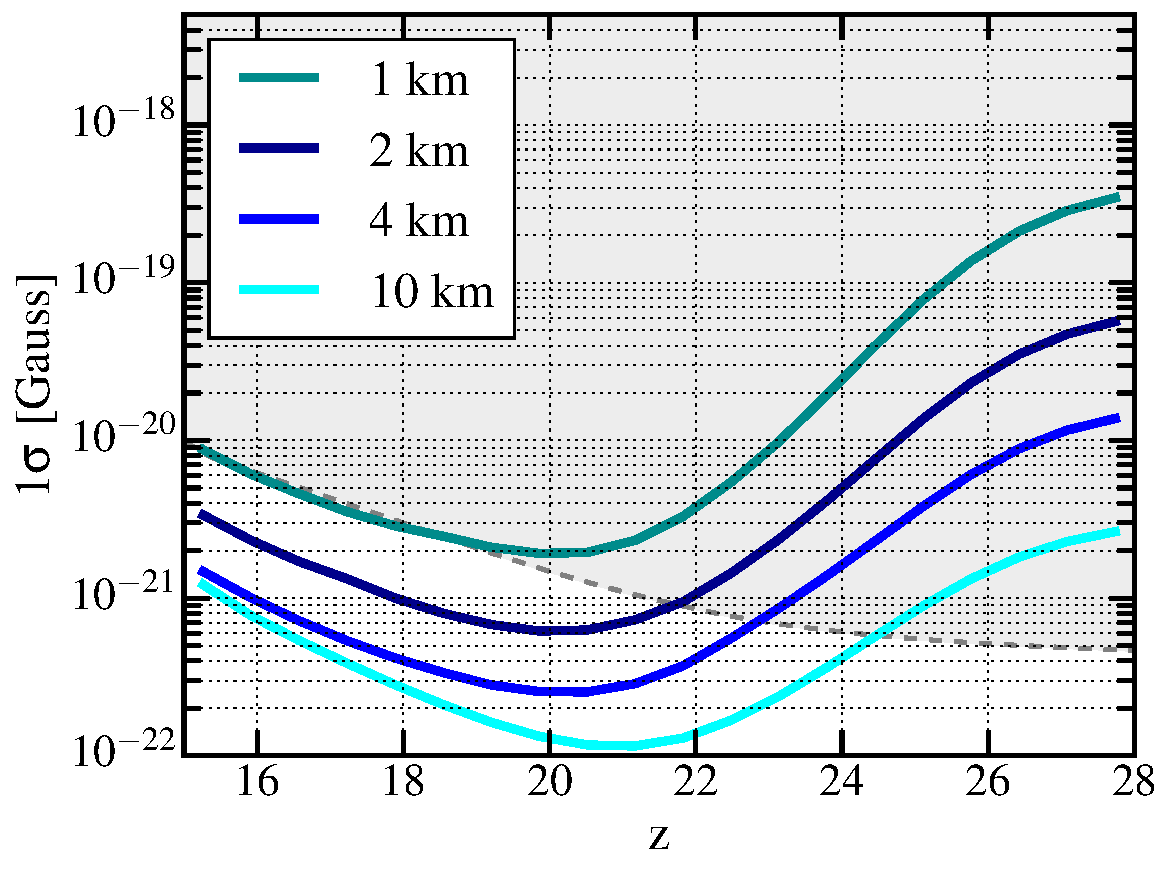
\includegraphics[width=.35\textwidth,keepaspectratio=true]{sigmaB0_vs_z.pdf}
\caption{Saturation regime is shown as a shaded gray area above the dashed curve (``saturation ceiling''). Integrand of \eq{\ref{eq:fisher_patch}} (inverse sqare root of it) is shown as a function of redshift, for several maximum---baseline lengths.  When the integrand values are close to the saturation ceiling, the analysis assuming unsaturated regime is valid. For the baseline lengths considered here, this is indeed the case for integrand values around their minima (corresponding to redshifts of maximal signal--to--noise for magnetic field detection), for arrays with collecting areas above a square kilometer; this implies that the corresponding projected sensitivities of Fig.~\ref{fig:B_vs_deltas} are valid. \label{fig:Bsat}}
\end{figure}
